\documentclass[UTF8]{article}
\usepackage{ctex}
\usepackage{ulem}
\usepackage{dsfont}
\usepackage{amssymb}
\usepackage{amsmath}
\usepackage{graphicx}
\newtheorem{thm}{定义}[section]
\newtheorem{notation}[thm]{记号}
\newtheorem{lemma}[thm]{引理}

\makeatletter
\newcommand{\rmnum}[1]{\romannumeral #1}
\newcommand{\Rmnum}[1]{\expandafter\@slowromancap\romannumeral #1@}
\makeatother
\newcommand{\dperp}{\perp\!\!\!\perp}

\title{12 $\lambda{\rm D}$中的数学:第一个尝试\\Mathematics in $\lambda{\rm D}$: a first attempt\\[2ex]\begin{large}读书笔记\end{large}}
\author{许博}
\date{}

\begin{document}
\maketitle
	\section{疑问}
		1. P260, Remark 12.2.1 中,为何定义$\Pi P:S\rightarrow*_p.(Px\Rightarrow Py)$也可以表示$x=y$?

	\section{先举个例子}
	\noindent
	第十一章中,我们在$\lambda{\rm D}$中表示了逻辑。在本章中,将转向数学(mathematics)。尽管逻辑的推导框架对数学至关重要,因为逻辑包含了推理的原则,但是数学本身要比单纯的逻辑多的多。
	
		本章以一个关于偏序集合的例子开始,即证明在这样的集合中只存在至多一个最小元。一个在集合$S$上的关系$R$如果满足自反性,反对称性和传递性,则这个关系是偏序的。\\
		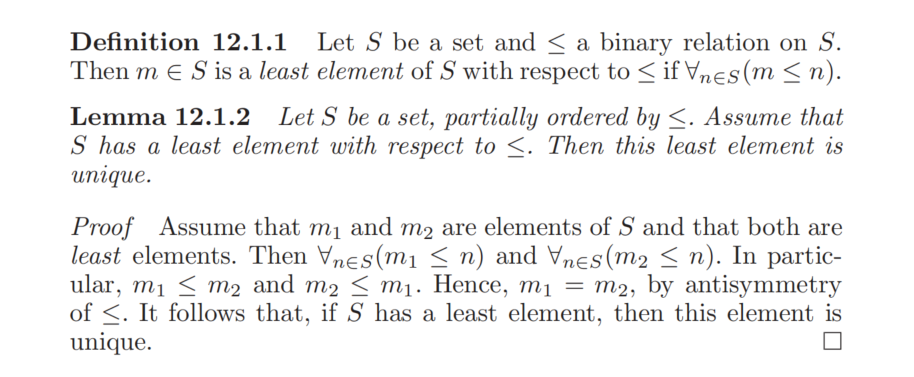
\includegraphics[width=0.93\linewidth]{"../imgs/12-1.png"}
		
		在$\lambda{\rm D}$中形式化这个证明:\\
		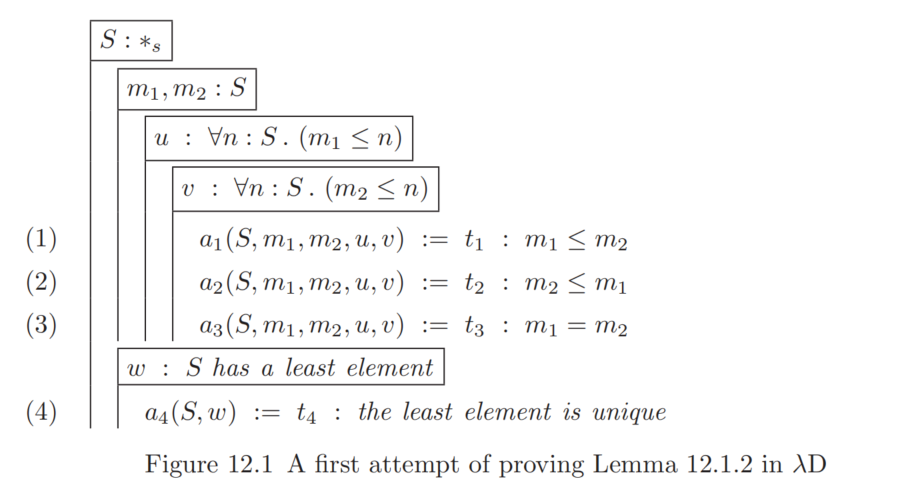
\includegraphics[width=0.93\linewidth]{"../imgs/12-2.png"}
		
		注意到其中存在的几个问题。有一些可以以直观的方式解决:\\
		- 符号`$\le$'表示在$S$上的一个任意的偏序关系。这些隐含的假设会在章节12.4中明确的表示。\\
		- 全称量词$\forall$在$\lambda{\rm D}$中被编码为$\Pi$。\\
		- 解决未知项$t_1$和$t_2$代表什么:应是$\forall$-消去规则的实例,所以令$t_1\equiv\forall{-el}(S,\lambda x:S.m_1\le x,u,m_2)$以及$t_2\equiv\forall{-el}(S,\lambda y:S.m_2\le y,v,m_1)$,或者简单地令$t_1\equiv um_2$以及$t_2\equiv vm_1$。
		
		剩下的问题似乎更加重要:\\
		$\it{Q1}$ 符号`='表示了基本的相等关系,作为数学中许多领域的基础,但尚未是我们系统的一部分,如何补足这点?\\
		$\it{Q2}$ 行(3)中$t_3$代表什么?\\
		$\it{Q3}$ 如何表达$S$拥有一个最小元?\\
		$\it{Q4}$ 如何表达最小元的唯一性?\\
		$\it{Q5}$ 如何证明最小元的唯一性,也即$t_4$是什么?
		
	\section{相等}
	\noindent
	相等显然是两个参数之间的关系:对于一对元素$x$和$y$,有命题$x=y$。又因为在类型理论中,每个元素都应具有一个类型;所以假设$S$是$x$和$y$的类型。故我们可以将相等看作是在$S$上的二元谓词。写作$x=_S y$以表示$S$中的$x$和$y$相等。
	
		所以,相等是一个参数化的二元关系:对每一个类型$S$,有一个相等关系$=_S:S\rightarrow S\rightarrow*$,作用于类型为$S$的项。
		
		现在,核心问题是:$S$中的元素$x$和$y$“相等”意味着什么?德国数学家莱布尼兹(G.W. Leibniz,1646-1716)给出的一个富有哲学的答案是,如果两个对象在所有可能的环境中都是不可分辨的,则这两个对象是相等的。可以更简洁地表示为:“对任意在$S$上的谓词$P$,$Px$的有效性等价于$Py$的有效性”,也即,对于给定的$P$,要么$Px$和$Py$都成立,要么两者都不成立。在这种情况下,没有可能分辨$x$和$y$,故两者相等。
		
		莱布尼兹对于相等的看法可以作为描述性定义在$\lambda{\rm D}$中进行形式化,形式化地定义$eq(S,x,y)$表示$S$中的元素$x$和$y$的相等,为
		
		$\Pi P:S\rightarrow*_p.(Px\Leftrightarrow Py)$
		
		甚至更为简单的定义也可以,即:
		
		$\Pi P:S\rightarrow*_p.(Px\Rightarrow Py)$
		
		使用图 12.2 显示这个被定义的相等时一个满足自反性的关系。使用名字$eq$-$refl(S,x)$表示自反性的证明。\\
		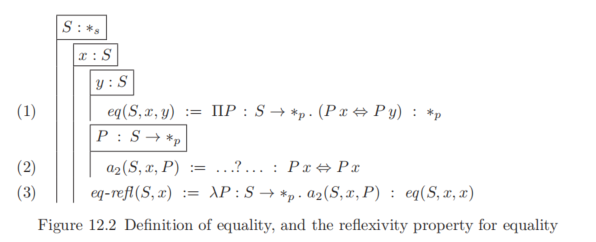
\includegraphics[width=0.93\linewidth]{"../imgs/12-3.png"}
		
		需要注意的是,我们得到的是相等的二阶定义,因为$\Pi$抽象的谓词$P:S\rightarrow*:\square$是二阶的,所以公式中的$\Pi$是一个二阶全称量词。
		
		在图 12.2 中的推导中存在一个空,即行(2)中,$Px\Leftrightarrow Px$的证明,有两种方式解决:
		
		(1) 特定的方法(ad-hoc approach):也即找到$Px\Leftrightarrow Px$的成员,使用表达式$\Leftrightarrow{-in}(Px,Px,\lambda u:Px.u,\lambda u:Px.u)$即可。
		
		(2) 通用方法:首先证明一个引理,即$A\Leftarrow A$对于任意的$A:*_p$都成立,命名这个证明为$\Leftrightarrow{-refl}(A)$,然后使用表达式$\Leftrightarrow{-refl}(Px)$填空即可。
		
		为便于阅读,使用记号$x=_S y$表示$eq(S,x,y)$。
		
		而相等还满足替代性(substitutivity),也即“对所有在$S$上的谓词$P$,如果$x=_S y$且$Px$成立,则$Py$”也成立,则当在任意命题中出现的$t_1$以及$t_1=_S t_2$,使用$t_2$替换$t_1$不影响命题的真值。\\
		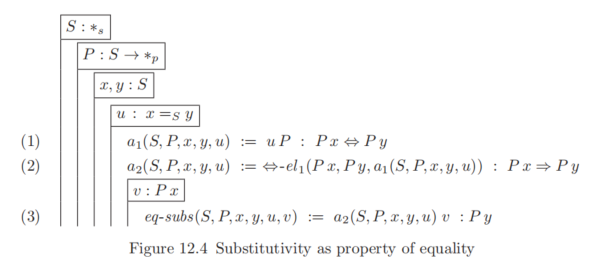
\includegraphics[width=0.93\linewidth]{"../imgs/12-4.png"}
		
	\section{相等的一致性}
	\noindent
	一致性与替代性相似,但一致性关注以集合而非命题作为域的函数。一致性即“对所有的函数$f:S\rightarrow T$且$x,y:S$,如果$x=_S y$,则$fx=_T fy$”。
	
		我们将使用$x=_S y$推导结果$fx=_T fy$,因此需要找到一个合适的谓词。首先展开目标$fx=_T fy$为$\Pi Q:T\rightarrow*_p.(Q(fx)\Leftrightarrow Q(fy))$。
		
		第一种方式,令谓词为$\lambda z:S.Q(fz)$,由替代性可以得到$Q(fy)$,证明过程如下:\\
		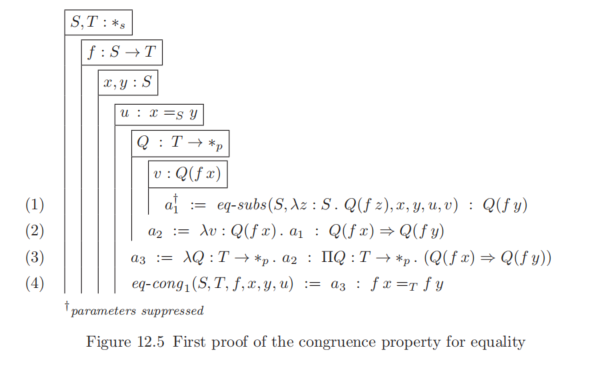
\includegraphics[width=0.93\linewidth]{"../imgs/12-5.png"}
		
		第二种方式,令谓词为$\lambda z:S.(fx=_T fz)$,由自反性可以得到$fx=_T fx$,再由替代性可以得到$fx=_T fy$,需要注意的是,第一个$x$是抽象中的自由变量,证明过程如下:\\
		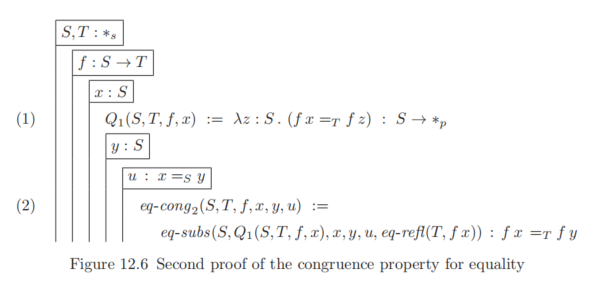
\includegraphics[width=0.93\linewidth]{"../imgs/12-6.png"}
		
	\section{序,Orders}
	\noindent
	在知道如何编码“相等”后,还需要知道引理 12.1.2 的证明中起到重要作用的其它关系,也即符号`$\le$'表示的序关系。与`='相似,$\le:S\rightarrow S\rightarrow*_p$,为了便于阅读,我们使用$x\le_S y$表示在集合$S$中的元素$x$和$y$上应用关系$\le$。形式化定义“偏序”(即偏序关系所具有的类型):\\
	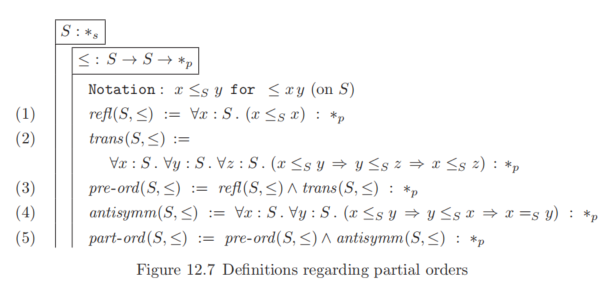
\includegraphics[width=0.93\linewidth]{"../imgs/12-7.png"}
	
		可以看到$\le$是具有自反性,传递性和反对称性的关系。
		
		现在可以证明由$x\le y\land y\le x\Rightarrow x=y$,也即图 12.1 中的 $t_3$:\\
		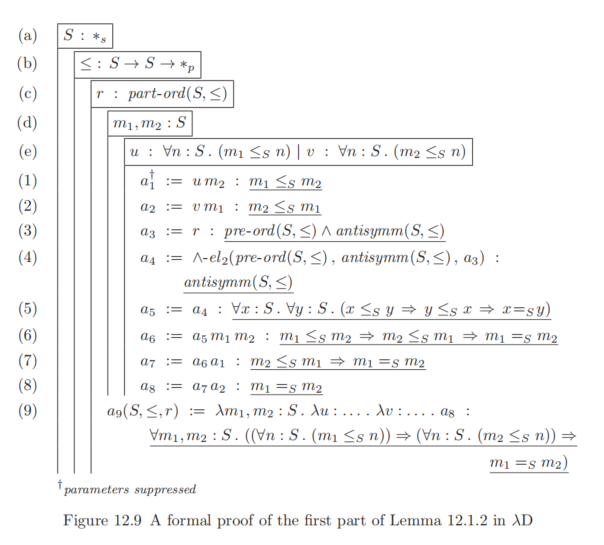
\includegraphics[width=0.93\linewidth]{"../imgs/12-8.png"}
		
		可以看到,证明主要依赖于偏序关系的反对称性。
		
	\section{关于序的证明}
	\noindent
	除了已经证明过的相等的自反性以及替代性外,还有对称性和传递性。
	
		对称性的证明使用了自反性和替代性:\\
		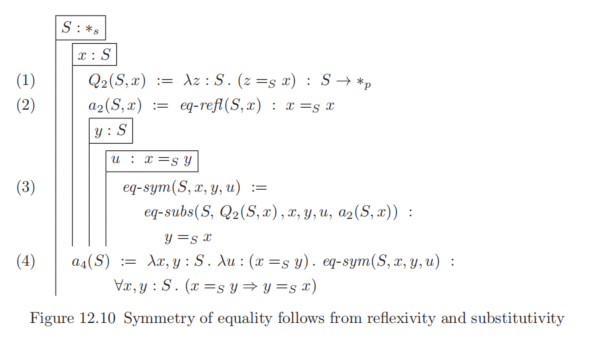
\includegraphics[width=0.93\linewidth]{"../imgs/12-9.png"}
		
		传递性的证明使用了替代性:\\
		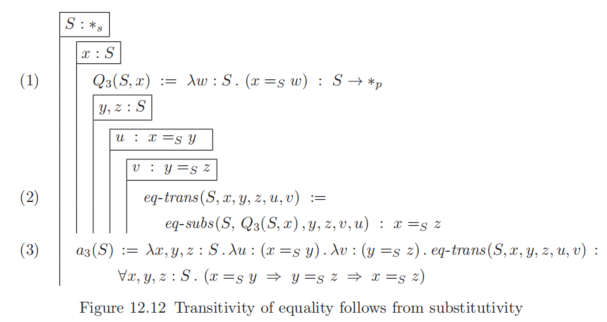
\includegraphics[width=0.93\linewidth]{"../imgs/12-10.png"}
\end{document}
